\section{AIC}


\begin{frame}{Accretion Induced Collapse (of White Dwarf)}

\begin{minipage}[t]{0.48\textwidth}
\vspace{0pt}
        \begin{figure}
                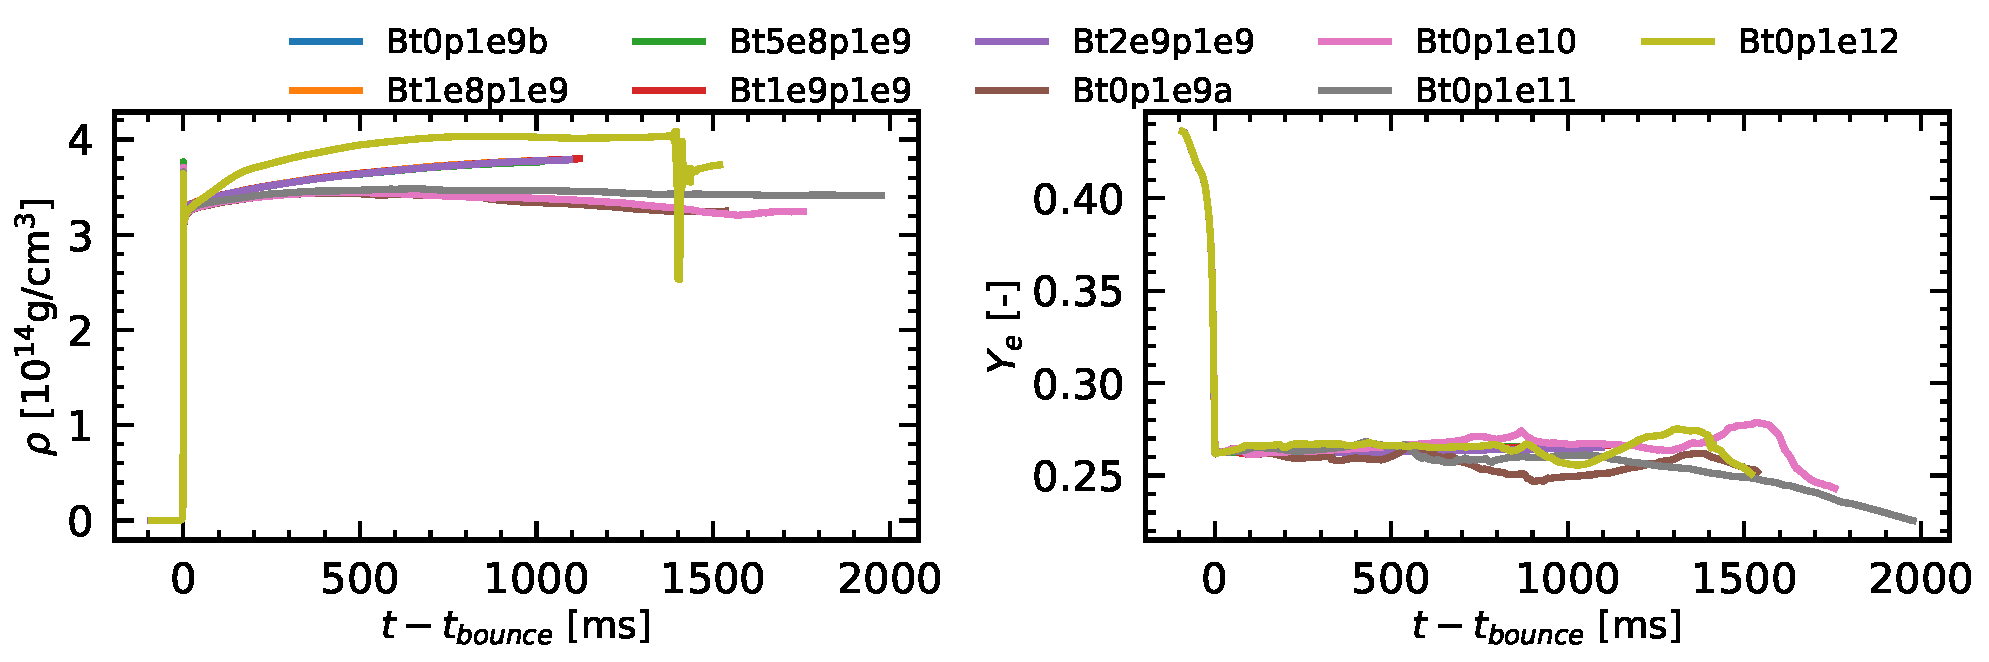
\includegraphics[width=1.1\linewidth]{../fig/AIC/Central_density_and_ye.pdf}
	      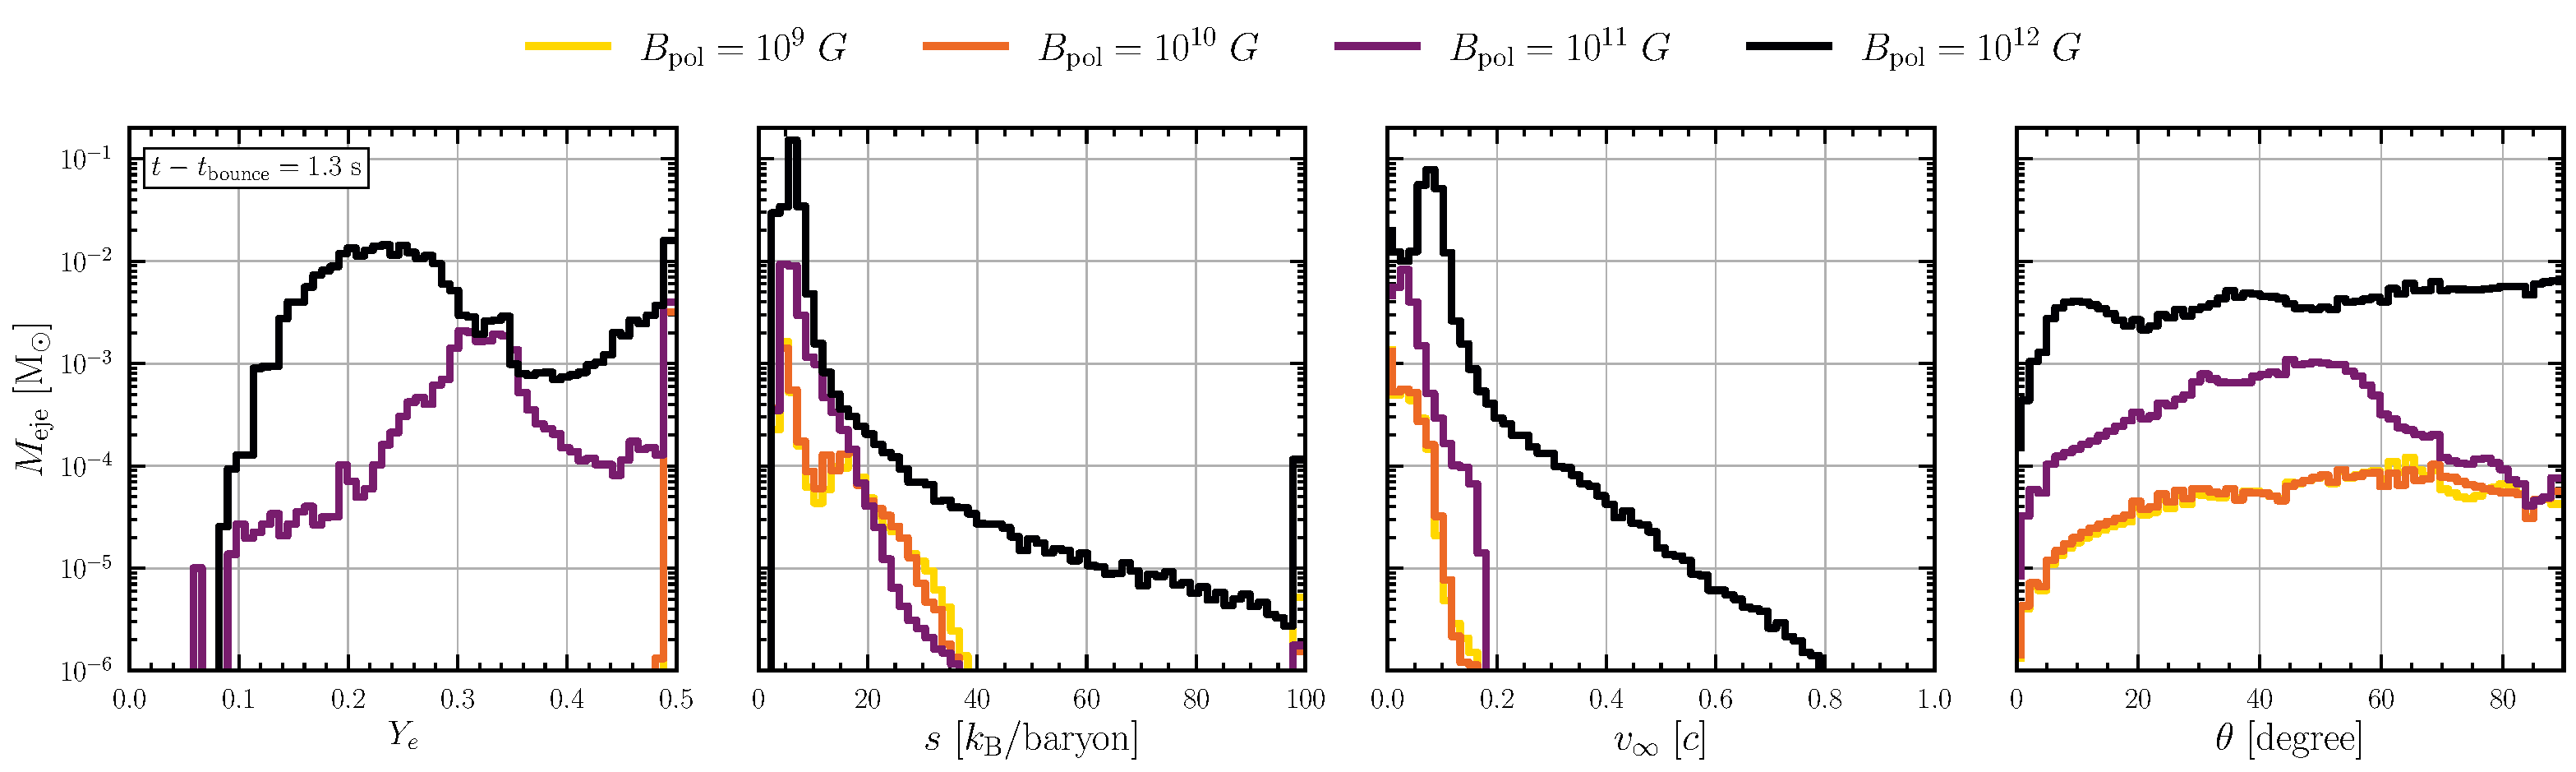
\includegraphics[width=1.1\linewidth]{../fig/AIC/fig_eje_histogram.pdf}
        \end{figure}

\end{minipage}
\hfill
\begin{minipage}[t]{0.45\textwidth}
\vspace{0pt}
\begin{tcolorbox}[
    colback=white,
    colframe=blue,
    colbacktitle=blue!50!black!50,
    title=Overview,
    fonttitle=\bfseries,
    rounded corners,
    boxrule=1pt,
    left=2mm, right=2mm, top=1mm, bottom=1mm
]
\begin{itemize}
   \scriptsize 
    \item WD with accretion history
    \item  $M\rightarrow  1.44 (1+\epsilon) M_{\odot}$ 
    \item  $Y_{e}\rightarrow Y_{e}(\rho)$ (until collapse) 
    \item M1 after collapse
    \item  MMA  (see 2306.04711)
    \item  LGRB + KN (see 2410.10938)
    \item magnetar formation (in prep.)
    \item Limitation: Isolated WD simulations (likely not true)

	
\end{itemize}
\end{tcolorbox}
\end{minipage}

\end{frame}


\begin{frame}{Questions}

\begin{minipage}[t]{0.48\textwidth}
\vspace{0pt}
        \begin{figure}
                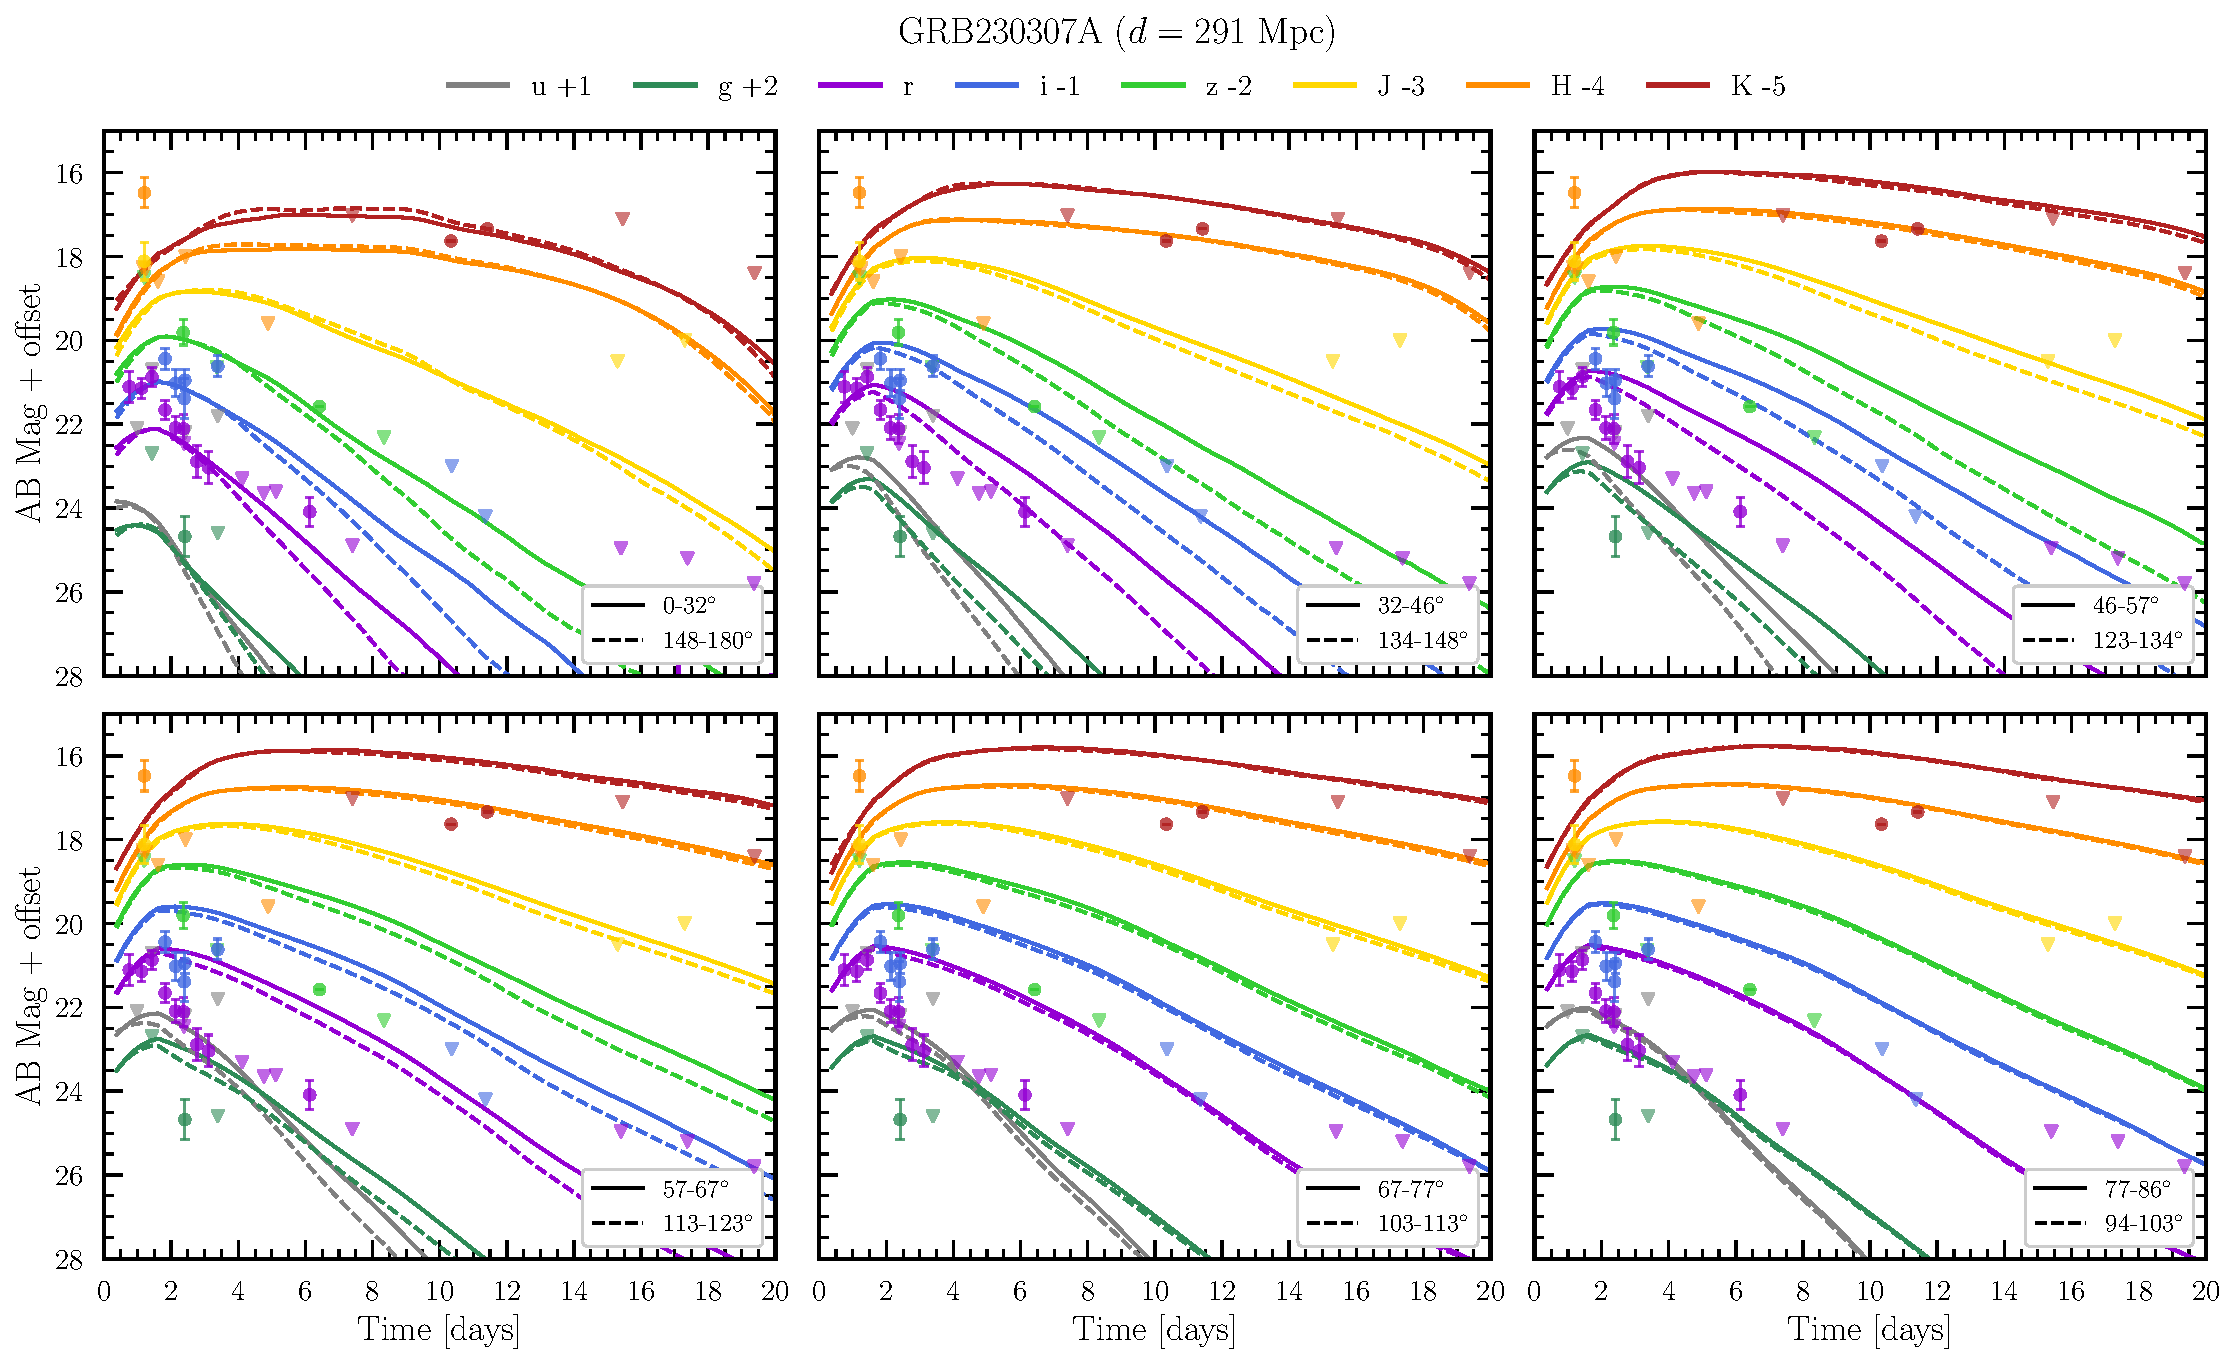
\includegraphics[width=1.1\linewidth]{../fig/AIC/H.pdf}

        \end{figure}

\end{minipage}
\hfill
\begin{minipage}[t]{0.45\textwidth}
\vspace{0pt}
\begin{tcolorbox}[
    colback=white,
    colframe=blue,
    colbacktitle=blue!50!black!50,
    title=Overview,
    fonttitle=\bfseries,
    rounded corners,
    boxrule=1pt,
    left=2mm, right=2mm, top=1mm, bottom=1mm
]
\begin{itemize}
   \scriptsize 
    \item WD with accretion history - Companion or disk
    \item WD may not accreate all mass before collapse
    \item Evolve ejecta of AIC with remans of companion
    \item Imprint on light curve or nucleosynthesis?
    \item Does it affect the aggreement foun with LGRB ? (see 2602.21291)
   \item Composition, mass, and distribution of the remains ?
	
\end{itemize}
\end{tcolorbox}
\end{minipage}

\end{frame}
